\documentclass[a4paper, 12pt]{scrartcl}
\usepackage[ngerman]{babel}
\usepackage[utf8]{inputenc}
\usepackage[T1]{fontenc}
\usepackage{lmodern}

\linespread{1.2}
\parindent0cm
\usepackage{graphicx}
\usepackage{hyperref}
\usepackage{float}
\usepackage{tabularx}
\usepackage{multicol}
\usepackage{units}
\usepackage{mathtools}

\usepackage{listings}
\usepackage{color}
\usepackage{geometry}
	\geometry{a4paper, top=25mm, left=20mm, right=20mm, bottom=30mm, headsep=10mm, footskip=12mm}
\usepackage{amssymb}
	

\lstset{literate=%
	{Ö}{{\"O}}1
	{Ä}{{\"A}}1
	{Ü}{{\"U}}1
	{ü}{{\"u}}1
	{ä}{{\"a}}1
	{ö}{{\"o}}1
	{█}{{$\blacksquare$}}1
	{~}{{\textasciitilde}}1
}

\definecolor{mygreen}{rgb}{0,0.6,0}
\definecolor{mygray}{rgb}{0.5,0.5,0.5}
\definecolor{mymauve}{rgb}{0.58,0,0.82}
\definecolor{deepred}{rgb}{0.6,0,0}

\lstset{ %
	backgroundcolor=\color{white},   % choose the background color; you must add \usepackage{color} or \usepackage{xcolor}; should come as last argument
	basicstyle=\scriptsize,          % the size of the fonts that are used for the code
	breakatwhitespace=false,         % sets if automatic breaks should only happen at whitespace
	breaklines=true,                 % sets automatic line breaking
	captionpos=b,                    % sets the caption-position to bottom
	commentstyle=\color{mygreen},    % comment style
	deletekeywords={...},            % if you want to delete keywords from the given language
	escapeinside={\%*}{*)},          % if you want to add LaTeX within your code
	extendedchars=true,              % lets you use non-ASCII characters; for 8-bits encodings only, does not work with UTF-8
	frame=single,	                 % adds a frame around the code
	keepspaces=true,                 % keeps spaces in text, useful for keeping indentation of code (possibly needs columns=flexible)
	keywordstyle=\color{blue},       % keyword style
	language=Python,                 % the language of the code
	morekeywords={*,...},            % if you want to add more keywords to the set
	emph={makevideo,checkgreen,checkblue,lenken,line,linienfahren,main},
	emphstyle=\color{deepred},
	numbers=left,                    % where to put the line-numbers; possible values are (none, left, right)
	numbersep=5pt,                   % how far the line-numbers are from the code
	numberstyle=\tiny\color{mygray}, % the style that is used for the line-numbers
	rulecolor=\color{black},         % if not set, the frame-color may be changed on line-breaks within not-black text (e.g. comments (green here))
	showspaces=false,                % show spaces everywhere adding particular underscores; it overrides 'showstringspaces'
	showstringspaces=false,          % underline spaces within strings only
	showtabs=false,                  % show tabs within strings adding particular underscores
	stepnumber=2,                    % the step between two line-numbers. If it's 1, each line will be numbered
	stringstyle=\color{mymauve},     % string literal style
	tabsize=2,	                     % sets default tabsize to 2 spaces
	title=\lstname                   % show the filename of files included with \lstinputlisting; also try caption instead of title
}
 
\begin{document}

\subsection{import}	%%%%%%%%%% import %%%%%%%%%%
\lstinputlisting[language=Python,firstline=1,lastline=14]{../main.py}

Am Anfang der Hauptdatei werden die benötigten Module importiert, gefolgt von den beiden ausgelagerten Dateien. Von aufrauemen.py werden nur die benötigten Funktionen importiert und von setup.py wird alles importiert, da diese Datei keine Funktion enthält.

In den Zeilen $10$ bis $14$ werden die benötigten Einstellungen für OpenCV 2 vorgenommen und ein erstes Bild aufgenommen.

\subsection{main}	%%%%%%%%%% main %%%%%%%%%%
\lstinputlisting[language=Python,firstline=167]{../main.py}

Das Programm wird in \textit{main} gestartet und beendet. Als erstes werden die Motoren mit der \text{losfahren} Funktion gestartet, allerdings noch mit einem Tastverhältnis von 0\%.
Anschließend wird das threading gestartet. Dafür wir wird \textit{run\_event}, das als \textit{while}-Bedingung für die threads dient, gesetzt. Die delay-Angaben und die drei verwendeten threads th1, th2 und th3 werden definiert. \textit{target} ist die Funktion die in dem neuen thread laufen soll und \textit{args} sind die Variablen die mit übergeben werden.
Die drei threads sind, \textit{linienfahren} (der eigentliche lenk-Algorithmus), \textit{checkblue} (der Test ob die Ampel blau leuchtet) und \textit{makevideo} (die Videoausgabe).\\

Der erste thread, die Videoaufzeichnung, wird gestartet. Dann folgt eine \textit{while}-Schleife die überprüft ob die Ampel grün ist. Wenn der zurückgegebene Wert der \textit{checkgreen} Funktion größer gleich 500 ist, also ausreichend Grünanteile erkannt wurden endet die Schleife. Dadurch werden die anderen beiden threads gestartet, wodurch das Auto losfährt.

Damit das Programm wieder beendet werden kann, folgt eine \textit{try-while} und \textit{except} Schleife, die weiter keine andere Funktion hat. Sobald ein \textit{KeyboardInterrupt} durch das drücken von Strg-c auftritt wird das Auto gebremst und die threads werden geschlossen. Allerdings muss dabei gewartet werden bis die \textit{while}-Schleifen aller threads durchgelaufen sind. Anschließend werden die GPIO einstellungen bereinigt, die Videoaufnahme beendet und das Video gespeichert.\\

Gestartet wird die \textit{main} Funktion durch eine \textit{if \_\_name\_\_ == "\_\_main\_\_"} abfrage, um die Datei auch als Modul verwenden zu können.



\subsection{line}	%%%%%%%%%% line %%%%%%%%%%
\lstinputlisting[language=Python,firstline=104,lastline=119]{../main.py}

In \textit{line} wird ein Bild aufgenommen und, in einer Zeile, der Mittelpunkt der roten Anteile ermittelt.

Der Funktion wird beim aufrufen die Zeile (\textit{zeileNr}) übergeben, die auf den Rotwert analysiert werden soll. Damit wird es ermöglicht die selbe Funktion zum analysieren unterschiedlicher Zeilen zu verwenden. Das wird in der finalen Version aber nicht benutzt.

In Zeile $12$ bis $16$ wird der Mittelpunkt berechnet und zurückgegeben. Falls kein Rotanteil über dem Schwellwert liegt, wird \textit{None} zurückgegeben.

\subsection{linienfahren}	%%%%%%%%%% linienfahren %%%%%%%%%%
\lstinputlisting[language=Python,firstline=122,lastline=164]{../main.py}

\textit{linienfahren} ruft die Funktion \textit{line} auf und berechnet die Lenkung und Geschwindigkeit aus dem zurückgegebenen Wert.

Am Anfang der Funktion wird ein Testbild aufgenommen und die für die Berechnung benötigten Variablen erstellt. Danach folgt eine \textit{while} Schleife, die bis zum Beenden des threading durchläuft.
Falls keine rote Linie im Bild war, oder in seltenen Fällen, wenn die Linie nicht erkannt wurde, gibt \textit{line} \textit{None} zurück. In diesem Fall wird, in den Zeilen $17$ bis $21$, überprüft ob die Linie zuletzt rechts oder links im Bild war. Der Messwert \textit{mitte} wird dementsprechend auf das Minimum (0) oder das Maximum (640) gesetzt. Anschließend wird der Wert für die Videoausgabe abgespeichert (Zeile $22$).

In den Zeilen $24$ bis $33$ wird der Wert für die Lenkung und Geschwindigkeit berechnet. Unterschieden wird zwischen drei Fällen. Ist der Messwert in der Mitte des Bildes wird geradeaus gelenkt, andernfalls wird die Lenkung und die Geschwindigkeit berechnet. Ist der Messwert größer als der Bildmittelpunkt wird $2-\textit{Lenkwert}$ gerechnet. Es ergibt sich ein Lenkwert zwischen 0 und 1 für eine Linkskurve und 1 bis 2 für eine Rechtskurve. Das hat den Vorteil, dass der \textit{lenken} Funktion nicht zusätzlich eine Richtungsangabe übergeben werden muss. Anschließend wird die \textit{lenken} Funktion mit den Lenk- und Geschwindigkeits-Variablen aufgerufen .\\

Der Wert für die Lenkung und die Geschwindigkeit wird aus dem Messwert und dem Bildmittelpunkt berechnet:
\begin{align}
	\text{Lenkung}&=\dfrac{\text{Messwert}}{\text{Bildmittelpunkt}}\cdot 90\% + 10\% \\
	\text{Geschwidigkeit}&=\dfrac{\text{Messwert}}{\text{Bildmittelpunkt}}\cdot 60\% + 40\%
\end{align}
Damit die Lenkung nicht zu stark ist, wird der Wert kleiner gewichtet ($\cdot 90\%$) und angehoben ($+10\%$). So startet der Wert nicht bei 0\% sondern bei 10\%.
Die Geschwindigkeit wird gleich berechnet, allerdings mit ($\cdot 60\%$) gewichtet und ($+40\%$) angehoben. Es wird also mit 60\% bis 100\% Geschwindigkeit gefahren.\\

Für die Text- und Videoausgabe wird die verstrichene Zeit berechnet.
Anschließend folgt in Zeile $40/41$ eine Textausgabe über die Konsole. Dabei werden $\frac{\textit{Messwert}}{10}$ Leerzeichen, dann ein Blockzeichen als Position des Messpunktes im Bild und die verbleibenden $64-\frac{\textit{Messwert}}{10}$ Leerzeichen geschrieben. Dann folgen noch Angaben zu Messpunkt, Lenkwert, Geschwindigkeit und Zeit. In der nächsten Zeile wird der Mittelpunkt mit einem Strich markiert. Es ergibt sich eine Textausgabe die zum Beispiel so aussieht:

\begin{lstlisting}[language=bash,basicstyle=\tiny,numbers=none]
               █                               x = 245.0 ;steer = 0.8 ;speed = 85.9 ;time = 00:00.00
                       |
                 █                             x = 265.0 ;steer = 0.8 ;speed = 89.7 ;time = 00:00.04
                       |
                   █                           x = 284.0 ;steer = 0.9 ;speed = 93.2 ;time = 00:00.08
                       |
                    █                          x = 292.0 ;steer = 0.9 ;speed = 94.8 ;time = 00:00.12
                       |
                     █                         x = 304.0 ;steer = 1.0 ;speed = 97.0 ;time = 00:00.16
                       |
                      █                        x = 312.0 ;steer = 1.0 ;speed = 98.5 ;time = 00:00.20
                       |
                       █                       x = 325.0 ;steer = 1.0 ;speed = 99.1 ;time = 00:00.24
                       |
\end{lstlisting}

\subsection{lenken}	%%%%%%%%%% lenken %%%%%%%%%%
\lstinputlisting[language=Python,firstline=76,lastline=101]{../main.py}

Die \textit{lenken} Funktion steuert das Tastverhältnis der Motoren. Übergeben werden zwei Parameter für die Lenkgewichtung und die Geschwindigkeit.
Am Anfang der Funktion werden einige Abfragen zur Fehlerverhütung vorgenommen, damit das Tastverhältnis nicht unter 0\% oder über 100\% liegt, dass würde sonst zu einem Absturz führen.\\
Damit das Auto in den Kurven nicht ungewollt langsamer fährt, wird ausgerechnet wie viel schneller sich die äußeren  Motoren drehen können.
\begin{align}
	\text{Kopfraum} = 100-\text{Geschwindigkeit}
\end{align}
Ist der Kopfraum größer als der Geschwindigkeitswert, wird der Kopfraum gleich der Geschwindigkeit gesetzt.\\

Die Tastverhältnisse der Motoren werden gleich dem Geschwindigkeitswert gesetzt, wenn der Lenkwert $steer=1$ ist. Sonst wird unterschieden ob der Lenkwert größer oder kleiner als 1 ist, um in die entsprechende Richtung zu lenken.
\begin{align}
	&\text{Innere Motoren:} &\text{Tastverhältnis} &= \text{Lenkwert}\cdot\text{Geschwindigkeit}\\
	&\text{Äußere Motoren:} &\text{Tastverhältnis} &= (1-\text{Lenkwert})\cdot\text{Kopfraum}+\text{Geschwindigkeit}
\end{align}
Die Kombination aus dem Lenkwert, Geschwindigkeitswert und Kopfraum ermöglicht ein stufenloses kurven fahren, ohne das an Geschwindigkeit verloren wird. Dabei ist es egal worauf die Werte basieren, es wird immer gleich sanft gelenkt.

\begin{table}[th!]
	\centering
	\caption{Beispielwerte für die Motorensteuerung}
	\begin{tabular}{c|c|c|c}
		Lenken & Geschwindigkeit & $T_{\text{innen}} [\%]$ &  $T_{\text{aussen}}[\%]$ \\ \hline 
		0,2 & 20 & \ 2 & 36 \\  
		    & 60 & 12  & 92 \\    
		    & 80 & 16  & 96 \\ \hline
		0,8 & 20 & 16  & 24 \\
		    & 60 & 48  & 68 \\
		    & 80 & 64  & 84 \\
	\end{tabular} 
\end{table}

\subsection{checkgreen}	%%%%%%%%%% checkgreen %%%%%%%%%%
\lstinputlisting[language=Python,firstline=36,lastline=50]{../main.py}

Die \textit{checkgreen} Funktion Analysiert ein ganzes Bild der Webcam auf ihren Grünanteil und gibt die Anzahl zurück.

\subsection{checkblue}	%%%%%%%%%% checkblue %%%%%%%%%%
\lstinputlisting[language=Python,firstline=53,lastline=73]{../main.py}

\textit{checkblue} funktioniert ähnlich wie \textit{checkblue}, allerdings läuft die Funktion in Dauerschleife und stoppt das Auto 1,5 Sekunden nachdem die blaue Ampel erkannt wurde.
Die Funktion nimmt dabei kein eigenes Bild auf, sondern verwendet das Bild, dass von den \textit{linienfahren} Funktion aufgenommen wurde. Beim starten des threads wird wartet die Funktion eine Sekunde, damit nicht die grüne Ampel fälschlicher weise als Stopsignal erkannt wird.

\subsection{makevideo}	%%%%%%%%%% mekvideo %%%%%%%%%%
\lstinputlisting[language=Python,firstline=17,lastline=33]{../main.py}

Die Aufgabe der \textit{makevideo} Funktion ist es die von der Kamera aufgenommenen Bilder als ein Video zu exportieren. Da das Video nur zur Fehleranalyse und Veranschaulichung dient, wird es vernachlässigt ob das Video in Echtzeit läuft. Dafür wird die aktuelle Fahrzeit, ab dem erkennen der grünen Ampel, unten links im Bild eingeblendet. Außerdem wird der zu dem Bild gehörende Messpunkt und dessen Wert eingezeichnet.

Das Video in Zusammenhang mit den eingeblendeten Werten ermöglicht eine deutlich bessere Fehleranalyse als eine Textausgabe über die Konsole (Abb.: \ref{schuh_im_bild}).

\begin{figure}[ht!] \centering
	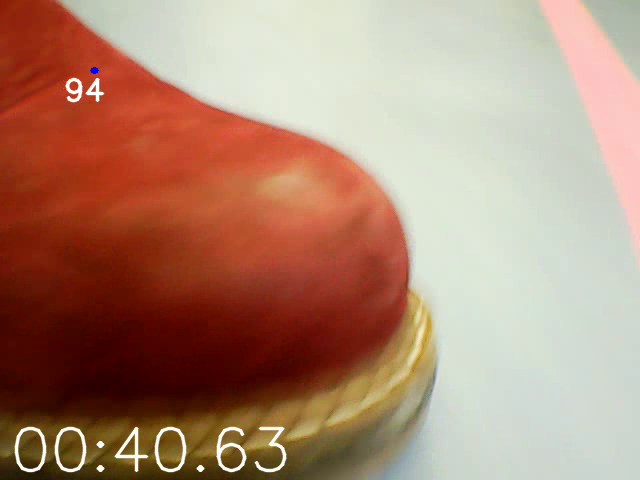
\includegraphics[width=.5\textwidth]{schuh_im_bild.png}
	\caption{Kamerabild mit Zeitanzeige und Messpunkt, abgelenkt von einem roten Schuh}
	\label{schuh_im_bild}
\end{figure}

\subsection{setup.py}	%%%%%%%%%% setup %%%%%%%%%%
\lstinputlisting[language=Python]{../setup.py}

In \textit{setup.py} werden die GPIOs definiert und wird am Anfang von \textit{main.py} aufgerufen. Verwendet wird der BCM Modus. Für die PWM wurde eine Frequenz von $\unit[73]{Hz}$ gewählt.

\subsection{aufraeumen.py}	%%%%%%%%%% aufräumen %%%%%%%%%%
\lstinputlisting[language=Python]{../aufraeumen.py}

In \textit{aufrauemen.py} sind drei Funktionen ausgelagert. \textit{losfahren} setzt die vier GPIOs der Motoren auf die entsprechenden Werte zum Vorwärtsfahren, \textit{bremsen} setzt die GPIOs, zum stoppen des Autos, auf null und \textit{aufrauemen} stoppt das Auto und bereinigt die GPIO Einstellungen.

\section{Anhang}

\subsection{main.py}
\lstinputlisting[language=Python]{../main.py}


\end{document}
